\section{Introduction}
\label{sec:section}
  Keyphrases are single or multi-word expressions that represent the main topics
  of a document. Keyphrases are useful in many tasks such as information
  retrieval~\cite{medelyan2008smalltrainingset}, document
  summarization~\cite{litvak2008graphbased} or document
  clustering~\cite{han2007webdocumentclustering}. Although scientific articles
  usually provide them, most of the documents have no associated keyphrases.
  Therefore, the problem of automatically assigning keyphrases to documents is
  an active field of research.

  Automatic keyphrase extraction methods are divided into two categories:
  supervised and unsupervised methods. Supervised methods typically recast
  keyphrase extraction as a binary classification
  task~\cite{witten1999kea,sujian2003maximumentropy,eichler2010keywe}. For
  unsupervised methods, keyphrase extraction is often considered as a ranking
  task and many approaches are
  used~\cite{barker2000nounphrasehead,tomokiyo2003languagemodel,mihalcea2004textrank}.
  As distinct as they are, both supervised and unsupervised methods rely on a
  preliminary candidate extraction step which identifies single and multi-word
  expressions that have the same syntactic properties than a keyphrase. These
  expressions are the only textual units that can be extracted as keyphrases.
  
  In this paper, we focus on the candidate extraction step and show its impact
  on the performance of automatic keyphrase extraction. Various methods
  are commonly employed to extract keyphrase candidates. Usually, a set of
  either single words, n-grams filtered by stop words, NP-chunks or sequences of
  words matching given patterns is extracted~\cite{hulth2003keywordextraction}.
  According to the chosen method, the extracted set contains more or less
  candidates, and the amount of these that match with the ground truth
  keyphrases may vary. Hence, a few questions arise. How the different sets
  influence the keyphrase extraction? Do large candidate sets introduce noise
  that affects the performance of some keyphrase extraction methods?

  We seek to better understand the impact of candidate extraction methods on
  keyphrase extraction by studying the aforementioned questions. We first
  quantify the differences between the candidate sets obtained by the commonly
  used methods. Also, we propose to use another method developed to extract
  noun-phrases for document indexing~\cite{evans1996nounphraseanalysis} and we
  argue that such term detection
  method~\cite{castellvi2001automatictermdetection} provides solid keyphrase
  candidates. Then, we evaluate the impact of the candidate extraction methods
  on three dissimilar keyphrase extraction methods. We select
  KEA~\cite{witten1999kea} to represent supervised methods,
  TF-IDF~\cite{jones1972tfidf} to represent unsupervised methods that require a
  collection of documents and TopicRank~\cite{bougouin2013topicrank} to
  represent unsupervised methods that only make use of the document to analyse.

  \todo[inline]{Results show that...}

\section{Candidate Extraction}
\label{sec:candidate_extraction}
  \todo[inline]{Objectif + pré-requis.}

  \subsection{Single Words Extraction}
  \label{subsec:single_words_extraction}
  \subsection{N-Gram Extraction}
  \label{subsec:n_gram_extraction}
  \subsection{NP-Chunk Extraction}
  \label{subsec:np_chunk_extraction}
  \subsection{Pattern Matching}
  \label{subsec:pattern_matching}
  \subsection{Term Extraction}
  \label{subsec:term_extraction}

\section{Keyphrase Extraction}
\label{sec:keyphrase_extraction}
  \todo[inline]{Fonctionnement général.}
  \begin{figure}
    \centering
    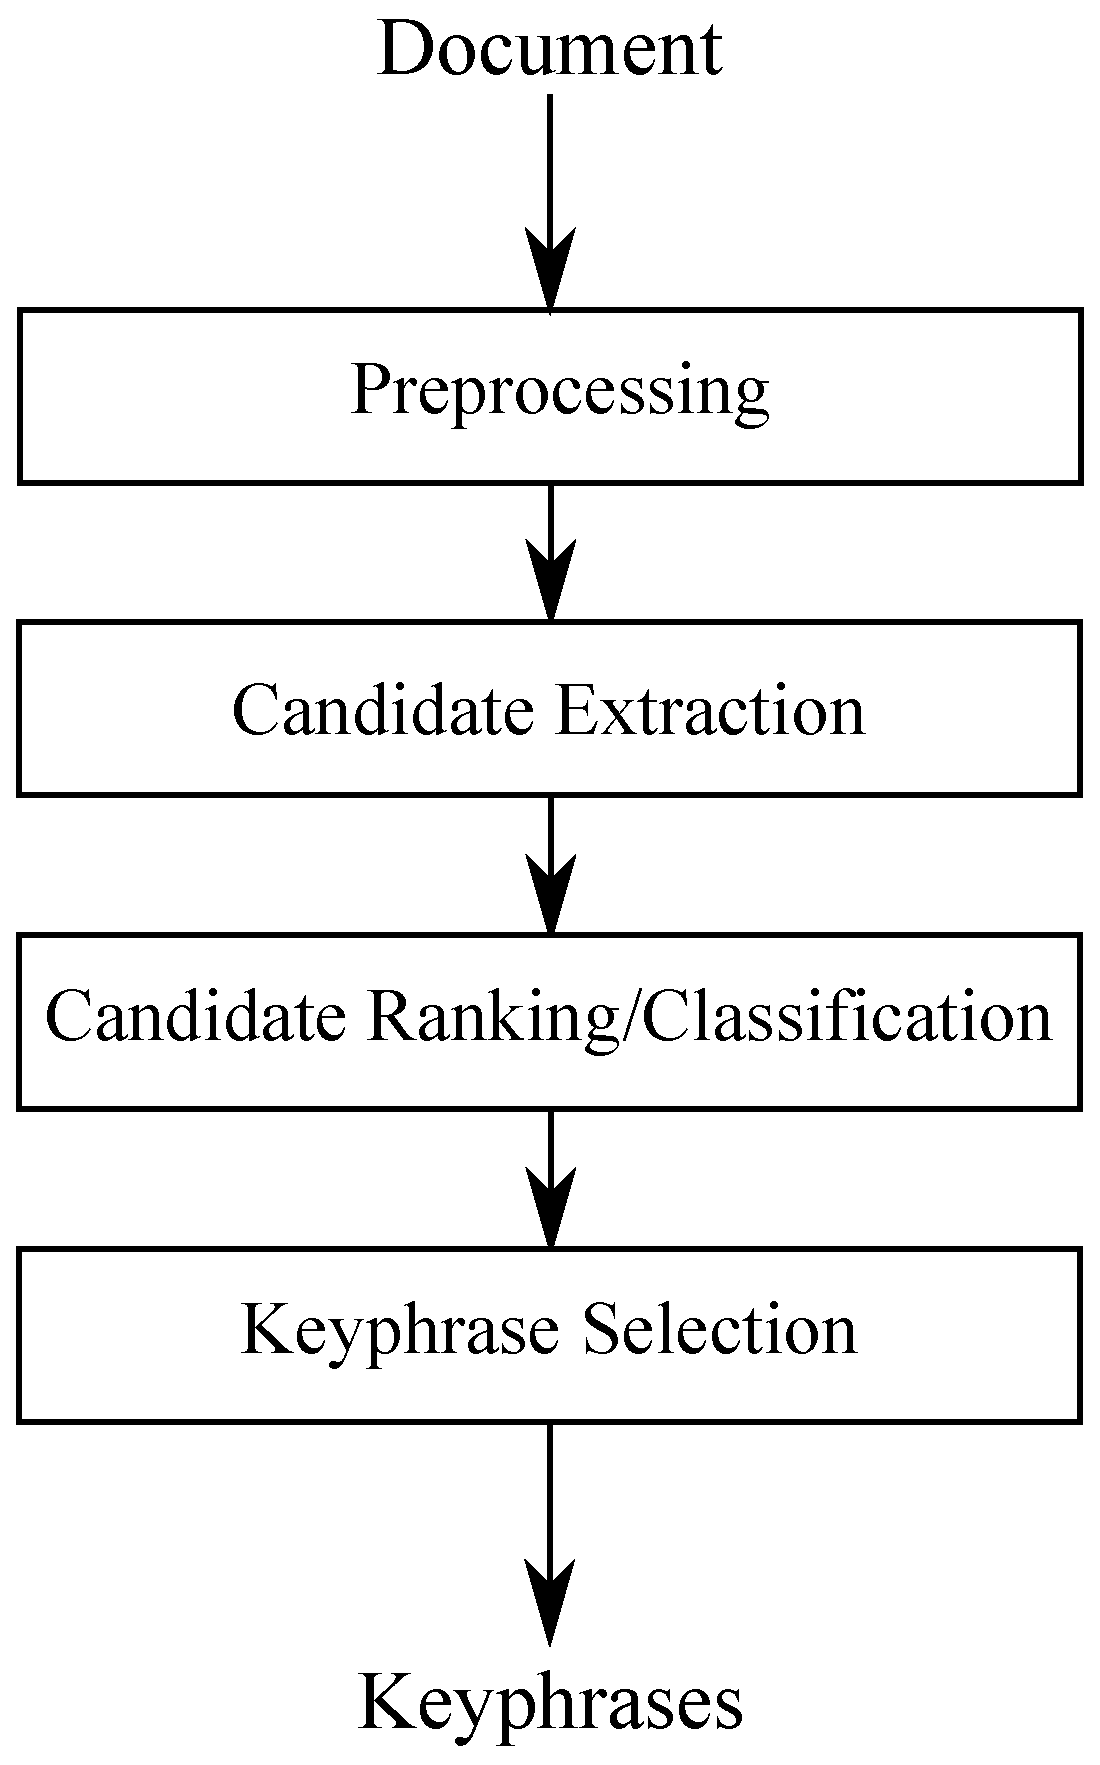
\includegraphics[width=0.3\textwidth]{include/processing_steps.eps}
    \caption{Processing steps of automatic keyphrase extraction methods.
             \label{fig:processing_steps}}
  \end{figure}

  \subsection{KEA}
  \label{subsec:kea}
  \subsection{TF-IDF}
  \label{subsec:tfidf}
  \subsection{TopicRank}
  \label{subsec:topicrank}

\section{Evaluation Datasets}
\label{sec:evaluation_datasets}
  \todo[inline]{Présentation générale des corpus pour l'extraction de
                termes-clés.}
  \todo[inline]{Présentation des corpus qui seront utilisés}

  \begin{table}[h]
    \centering
    \begin{tabular}{@{~}r@{~~}r@{~~}c@{~~}c@{~}}
      \toprule
      \multicolumn{2}{c}{\multirow{2}{*}[-2pt]{\textbf{Statistics}}} & \multicolumn{2}{c}{\textbf{Corpora}}\\
      \cmidrule{3-4}
      & & DUC & SemEval\\
      \midrule
      \multirow{5}{*}[-2pt]{\begin{sideways}\textbf{Documents}\end{sideways}} & Type & News & Papers\\
      & Documents & 308 & 100\\
      & Tokens/document & & 5176.6\\
      & Keyphrases/document & & 14.7\\
      & Missings keyphrases & & 19.3\%\\
      \addlinespace[\defaultaddspace]
      \multirow{10}{*}[-2pt]{\begin{sideways}\textbf{Keyphrases}\end{sideways}} & Unigrams & & \\
      & Bigrams & & \\
      & Trigrams and more & & \\
      & Containing nouns & & \\
      & Containing adjectives & & \\
      & Containing verbs & & \\
      & Containing adverbs & & \\
      & Containing prepositions & & \\
      & Containing determiners & & \\
      & Containing others & & \\
      \bottomrule
    \end{tabular}
    \caption{Dataset statistics. The missing keyphrase percentage is determined
             based on the stemmed form of the gold standard keyphrases.
             \label{tab:dataset_statistics}}
  \end{table}

  \todo[inline]{Donner les séquences de POS les plus fréquentes dans le gold
                standard.}

\section{Evaluation}
\label{sec:evaluation}
  \todo[inline]{Expliquer les deux évaluations: intrinsèque et extrinsèque.}

  \subsection{Experimental Setting}
  \label{subsec:experimental_setting}

  \subsection{Candidate Extraction}
  \label{subsec:candidate_extraction}
    \todo[inline]{Reprendre les statistiques données en
                  section~\ref{sec:evaluation_datasets}, pour les termes
                  candidats extraits.}
    \todo[inline]{Donner le rappel max et comparer avec la taille des différents
                  ensemble.}
    \todo[inline]{Quels sont les termes candidats communs aux ensembles, le
                  propriétés ?}

  \subsection{Keyphrase Extraction}
  \label{subsec:keyphrase_extraction}
    \todo[inline]{Quelles sont les performances de chaque méthode avec chaque
                  ensemble de termes candidats ?}
    \todo[inline]{Que se passe-t-il lorsque l'on ajoute les termes-clés manquant
                  (mais présents dans le document) aux termes candidats (càd
                  comment les termes candidats non termes-clés de chaque
                  ensemble influent sur les résultats)?}

